\documentclass[10pt,twocolumn,letterpaper]{article}

\usepackage[utf8]{inputenc}
\usepackage[T1]{fontenc}
\usepackage{lmodern}
\usepackage[margin=0.72in,top=0.80in,bottom=0.80in]{geometry}
\usepackage{amsmath,amssymb,amsfonts,bm}
\usepackage{graphicx}
\usepackage{booktabs}
\usepackage{tabularx}
\usepackage{multirow}
\usepackage{xcolor}
\usepackage{hyperref}
\usepackage[expansion=false]{microtype}
\usepackage{siunitx}
\usepackage{fancyhdr}
\usepackage{titlesec}
\usepackage{enumitem}
\usepackage{caption}
\usepackage{float}
\usepackage{tcolorbox}
\emergencystretch 1.5em

\graphicspath{{figures/}{paper/figures/}{../../outputs/scientific_study_verified/advanced_capabilities/figures/}{../../outputs/scientific_study_verified/figures/}}

\definecolor{navyblue}{RGB}{12, 35, 64}
\definecolor{accentteal}{RGB}{0, 132, 168}
\definecolor{darkgray}{RGB}{45, 52, 64}
\definecolor{panelbg}{RGB}{246, 248, 252}
\definecolor{panelborder}{RGB}{200, 212, 226}

\hypersetup{
    colorlinks=true,
    linkcolor=navyblue,
    citecolor=accentteal,
    urlcolor=accentteal,
    pdftitle={Earth-2 X-Band SAR and InSAR Mission Twin: Engineering Report},
    pdfauthor={Zhane Daye}
}

\pagestyle{fancy}
\fancyhf{}
\fancyhead[L]{\footnotesize\textcolor{darkgray}{\textbf{Earth-2 X-Band SAR \& InSAR Mission Twin} $|$ Engineering Report}}
\fancyhead[R]{\footnotesize\textcolor{darkgray}{Zhane Daye --- SAR \& Earth System Engineering}}
\fancyfoot[L]{\footnotesize\textcolor{darkgray}{\url{https://earth2-sar-insar.vercel.app} $|$ \url{https://github.com/zrt219/earth2studio}}}
\fancyfoot[R]{\footnotesize\textcolor{darkgray}{\textbf{Page \thepage}}}
\renewcommand{\headrulewidth}{0.4pt}
\renewcommand{\footrulewidth}{0.4pt}

\titleformat{\section}{\large\bfseries\color{navyblue}}{\thesection}{0.7em}{}[\titlerule]
\titleformat{\subsection}{\normalsize\bfseries\color{accentteal}}{\thesubsection}{0.6em}{}
\titleformat{\subsubsection}{\small\bfseries\color{darkgray}}{\thesubsubsection}{0.5em}{}

\title{\vspace{-0.8cm}\textbf{\LARGE Earth-2 X-Band SAR \& InSAR Mission Twin: Operational Tropospheric Phase Screen Compensation, Flood Backscatter Attribution, and Autonomous STAC Tasking}\\
\vspace{0.2cm}
\large\textit{Coupling Verified NOAA GFS $0.25^\circ$ Atmospheric Analyses with X-Band ($9.65\text{ GHz}$) Synthetic Aperture Radar Physics in an Interactive 3D WebGL Digital Twin (\url{https://earth2-sar-insar.vercel.app})}}

\author{
    \textbf{Zhane Daye}\\
    \textit{SAR \& Earth System Engineering $|$ Edmonton, AB, Canada}\\
    \small \texttt{zhanedaye@umattr.ca} \quad $|$ \quad \href{https://www.linkedin.com/in/zhane-umattr}{linkedin.com/in/zhane-umattr} \quad $|$ \quad \href{https://github.com/zrt219/earth2studio}{github.com/zrt219/earth2studio}\\
    \small \textbf{Live 3D WebGL Mission Twin:} \url{https://earth2-sar-insar.vercel.app}
}
\date{November 2026}

\begin{document}

\maketitle
\thispagestyle{fancy}

\begin{abstract}
\noindent
Commercial X-band ($f_c = 9.65\text{ GHz}$, $\lambda = 3.1067\text{ cm}$) Synthetic Aperture Radar (SAR) constellations---specifically \textbf{ICEYE} and \textbf{Synspective (StriX)}---deliver sub-meter to 3-meter all-weather Earth observation for rapid flood disaster response and millimetric infrastructure deformation monitoring. However, X-band Interferometric SAR (InSAR) is acutely sensitive to turbulent lower-tropospheric water vapor and hydrostatic stratification: a mere $1.5533\text{ cm}$ ($\lambda/2$) two-way slant-range path delay induces a full $2\pi$ interferometric phase wrap, masking millimeter-scale surface subsidence and pre-landslide slope creep beneath $8\text{--}15$ atmospheric fringes. Furthermore, agile constellation tasking requires automated Tip-and-Cue pipelines that translate synoptic Numerical Weather Prediction (NWP) and AI-NWP hazard forecasts into standards-compliant satellite acquisition orders before storm landfall.

This engineering report presents the design, physical formulation, numerical verification, and production deployment of the \textbf{Earth-2 X-Band SAR \& InSAR Mission Twin Web Application} (\texttt{viewer\_app/}, deployed live at \url{https://earth2-sar-insar.vercel.app}). Built upon an audited, leakage-free 3-stage atmospheric verification pipeline (\textbf{Forecast $\to$ Freeze $\to$ Verify}) operating on authentic NOAA GFS $0.25^\circ$ global analyses ($721 \times 1440$), the interactive digital twin integrates:
(1) a \textbf{CATALYST-grade X-Band Tropospheric Atmospheric Phase Screen (APS)} forward and inverse compensation engine using $8\times$ mesoscale Nyquist-resolved ($0.03125^\circ \approx 3.4\text{ km}$) Saastamoinen hydrostatic and Askne--Nordius wet refractivity integration, achieving a \textbf{98.73\% phase RMSE reduction} ($14.7763 \to 0.1874\text{ rad}$, $12.20$ fringes removed) over Northern Italy/Alps and a \textbf{98.81\% phase RMSE reduction} ($13.8243 \to 0.1641\text{ rad}$, $9.24$ fringes removed) over Central Honshu, Japan;
(2) \textbf{ICEYE X-band VV flood backscatter ($\sigma^0_{\text{VV}}$)} forward modeling delineating $735.27\text{ km}^2$ of specular riverine inundation ($\sigma^0_{\text{VV}} < -16.5\text{ dB}$, minimum $-31.77\text{ dB}$) in the Po Valley;
(3) \textbf{Synspective StriX-3 interferometric coherence ($\gamma_{\text{CCD}}$)} decay attribution isolating $550.73\text{ km}^2$ of severe topographic phase decorrelation ($\gamma < 0.32$, minimum $0.080$) during Typhoon Megi passage;
(4) an \textbf{OGC STAC v1.0.0 SAR Tasking Generator} with cryptographic SHA-256 provenance;
(5) an enterprise \textbf{Three.js 3D WebGL Digital Twin} featuring 16K global octant and 131K regional Sentinel-2 tiled LOD streaming with an $81\%$ GPU memory optimization ($1.29\text{ GiB} \to 248\text{ MB}$ VRAM); and
(6) an exhaustive multi-tier verification harness consisting of 321 Pytest checks, 105 WebGL E2E tests, 25 GEOINT SAR integration assertions, and automated Chrome DevTools Protocol (CDP) verification across desktop, tablet, and mobile viewports.
\end{abstract}

\section{Executive System Architecture \& Industry Alignment}

Modern operational remote sensing ground segments bridge two historically separated disciplines: global atmospheric modeling (NWP / AI-NWP) and coherent microwave radar observation. When extreme cyclogenesis or baroclinic fronts impact complex relief, atmospheric thermodynamics simultaneously drive destructive surface hazards (inundation, slope failure) while corrupting the microwave propagation path used to quantify them.

The \textbf{Earth-2 X-Band SAR \& InSAR Mission Twin Web Application} (\url{https://earth2-sar-insar.vercel.app}) functions as the interactive operational cockpit uniting these physics. Table~\ref{tab:industry_alignment} summarizes how the engineered subsystems align with commercial SAR constellations and enterprise InSAR processing suites.

\begin{table*}[t]
\centering
\footnotesize
\setlength{\tabcolsep}{4.5pt}
\caption{System Architecture Alignment with Commercial SAR Constellations and Enterprise InSAR Workflows}
\label{tab:industry_alignment}
\vspace{0.1cm}
\begin{tabularx}{\textwidth}{>{\raggedright\arraybackslash}p{2.8cm} >{\raggedright\arraybackslash}p{3.5cm} >{\raggedright\arraybackslash}p{5.1cm} >{\raggedright\arraybackslash}X}
\toprule
\textbf{Target Organization} & \textbf{Engineered Module} & \textbf{Physical \& Algorithmic Implementation} & \textbf{Verified Quantitative Performance} \\
\midrule
\textbf{CATALYST} \newline \textit{(PCI Geomatics / InSAR)} & \texttt{sar\_geoint\_engine.py} \newline \texttt{sarTasking.js} & Two-way X-band ($9.65\text{ GHz}$) tropospheric path delay integration ($\text{ZHD} + \text{ZWD}$) with $8\times$ bicubic mesoscale upsampling ($0.03125^\circ$) and hydrostatic scale filtering ($\sigma = 1.8$ coarse cells) for DEM-coupled APS removal. & \textbf{Italy/Alps:} $98.73\%$ RMSE reduction ($14.7763 \to 0.1874\text{ rad}$), $12.20$ fringes removed. \newline \textbf{Japan/Honshu:} $98.81\%$ RMSE reduction ($13.8243 \to 0.1641\text{ rad}$), $9.24$ fringes removed. \\
\addlinespace[0.12cm]
\textbf{ICEYE} \newline \textit{(X-Band SAR Constellation)} & \texttt{sar\_geoint\_engine.py} \newline \texttt{sarTasking.js} & \textbf{ICEYE-X38} ascending pass ($i = 97.7^\circ$ SSO, $\theta_{\text{inc}} = 28.4^\circ$, $0.5\text{ m}$ Spotlight VV) forward backscatter model ($\sigma^0_{\text{VV}}$) for specular open-water flood segmentation and Bragg capillary wind roughening. & Delineates \textbf{$735.27\text{ km}^2$} ($1,380$ mesoscale pixels) of Po Valley riverine flood inundation below $-16.5\text{ dB}$ ($\sigma^0_{\text{VV,min}} = -31.77\text{ dB}$ vs.\ $-7.71\text{ dB}$ land mean). \\
\addlinespace[0.12cm]
\textbf{Synspective} \newline \textit{(StriX Constellation)} & \texttt{sar\_geoint\_engine.py} \newline \texttt{sarTasking.js} & \textbf{StriX-3} descending pass ($i = 97.6^\circ$ SSO, $\theta_{\text{inc}} = 34.1^\circ$, $3.0\text{ m}$ StripMap VV/VH) repeat-pass Coherent Change Detection ($\gamma_{\text{CCD}}$) coupling wind/moisture volume decorrelation with steep slope geometry. & Identifies \textbf{$550.73\text{ km}^2$} ($5,294$ mesoscale pixels) of high-risk Honshu mountain slope decorrelation ($\gamma_{\text{CCD}} < 0.32$, $\gamma_{\text{min}} = 0.080$, land mean $\bar{\gamma} = 0.786$). \\
\addlinespace[0.12cm]
\textbf{Mission Operations} \newline \textit{(Tip-and-Cue Ground Segment)} & \texttt{sar\_geoint\_engine.py} \newline \texttt{uiController.js} & Automated anomaly-to-tasking translator exporting OGC STAC v1.0.0 \texttt{FeatureCollection} GeoJSON with \texttt{sar:*} extensions and interactive 3D WebGL orbital frustums. & 2 valid STAC v1.0.0 tasking orders (\texttt{ICEYE-X38}, \texttt{StriX-3}) sealed with SHA-256 digest \texttt{3fecc248...0d47035}; 1-click browser GeoJSON export. \\
\bottomrule
\end{tabularx}
\end{table*}

\section{Scientific Provenance: Real Operational Data vs.\ Forward-Modeled SAR Physics}

A core foundational discipline of this engineering initiative (enforced via repository governance rule \texttt{e2s-014-scientific-integrity.mdc} and verified through automated AST parsing) is the uncompromising separation between \textbf{authentic operational meteorological observations}, \textbf{deterministic physical forward operators}, and \textbf{forward sensor simulations}. Table~\ref{tab:provenance_boundaries} documents the provenance demarcation of every subsystem.

\begin{table*}[t]
\centering
\footnotesize
\setlength{\tabcolsep}{4.5pt}
\caption{Provenance Demarcation: Real Operational Observations vs.\ Deterministic Forward-Modeled SAR Physics}
\label{tab:provenance_boundaries}
\vspace{0.1cm}
\begin{tabularx}{\textwidth}{>{\raggedright\arraybackslash}p{3.6cm} >{\raggedright\arraybackslash}p{3.2cm} >{\raggedright\arraybackslash}p{4.7cm} >{\raggedright\arraybackslash}X}
\toprule
\textbf{Subsystem / Artifact} & \textbf{Provenance Tier} & \textbf{Physical Data Source / Input Tensors} & \textbf{Scope \& Validation Limitations} \\
\midrule
\textbf{Global $T_{2m}$ Initial \& Verifying States} \newline (\texttt{initial\_condition.npy}, \texttt{verifying\_truth\_t2m.npy}) & \textcolor{navyblue}{\textbf{Real Operational Analysis}} & Authentic NOAA Global Forecast System (GFS) $0.25^\circ$ operational gridded analyses ($721 \times 1440$, $1,038,240$ grid points) ingested via Earth2Studio. & Verified via 3-stage Forecast--Freeze--Verify protocol with SHA-256 manifest sealing. Baseline 24h persistence $\text{RMSE}_w = 2.1290\text{ K}$, $\text{MAE}_w = 1.0369\text{ K}$. \\
\addlinespace[0.10cm]
\textbf{Tropospheric Zenith \& Slant Delays} \newline ($\text{ZHD}$, $\text{ZWD}$, $\text{ZTD}$, $\Delta\phi_{\text{APS}}$) & \textcolor{accentteal}{\textbf{Deterministic Forward Physics on Real GFS}} & Driven directly by verified NOAA GFS $T_{2m}$ and 24h tendency $\Delta T_{2m}$ fields coupled with regional digital elevation relief $h(\phi,\lambda)$ and Clausius--Clapeyron vapor pressure $e(T, \text{RH})$. & Uses Saastamoinen hydrostatic and Askne--Nordius wet refractivity integration. Represents a physical NWP-to-InSAR forward operator rather than raw Level-1 SLC radar echoes. \\
\addlinespace[0.10cm]
\textbf{Mesoscale $8\times$ Nyquist Grid Upsampling} \newline ($0.25^\circ \to 0.03125^\circ$) & \textcolor{accentteal}{\textbf{Numerical PDE / Spline Downscaling}} & $8\times$ bicubic spline refinement ($\text{order}=3$) of GFS thermodynamic states with environmental lapse-rate topography ($\Gamma = 6.5\text{ K/km}$). & Required to resolve steep X-band phase gradients ($\lvert\nabla\phi\rvert < \pi\text{ rad/pixel}$) without spatial aliasing across $0.25^\circ$ ($\sim 27.8\text{ km}$) coarse NWP grid cells. \\
\addlinespace[0.10cm]
\textbf{SAR Flood Backscatter \& InSAR Coherence} \newline ($\sigma^0_{\text{VV}}$, $\gamma_{\text{CCD}}$) & \textcolor{accentteal}{\textbf{Forward Sensor Simulation}} & Parameterized physical forward models driven by GFS boundary-layer forcing, topographic slope $\lVert\nabla h\rVert$, and hydrological accumulation zones. & Demonstrates mission-planning Tip-and-Cue attribution and 3D Digital Twin visualization; not a substitute for calibrated Level-1B GRD/SLC satellite imagery. \\
\addlinespace[0.10cm]
\textbf{Hardware \& Prognostic Execution Scope} & \textcolor{darkgray}{\textbf{Documented Hardware Boundary}} & Executed on Windows 11 host with AMD Ryzen / Radeon hardware (no local NVIDIA CUDA tensor cores). & Local neural weights (FourCastNet, SFNO, GraphCast) require CUDA; live cloud inference was verified via NVIDIA Earth-2 Hosted API (\texttt{fourcastnet\_hosted.py}). \\
\bottomrule
\end{tabularx}
\end{table*}

\subsection{Three-Stage Anti-Leakage Architecture}
Prior to building the SAR/InSAR forward physics layer, an audit identified an unphysical historical synthetic formula ($\hat{y} = x_0 + 0.72(y_{\text{truth}} - x_0) + \epsilon$) that exhibited look-ahead target leakage. We eliminated and quarantined this defect, restructuring the workflow into three cryptographically isolated execution stages:
\begin{enumerate}[leftmargin=*,noitemsep,topsep=2pt]
    \item \textbf{Stage A --- Pure Forecast (\texttt{forecast\_stage.py}):} Ingests exclusively initial analysis $X(t_0)$ and predicts state $\hat{Y}(t_0 + \Delta t)$ in strict memory isolation prior to loading truth.
    \item \textbf{Stage B --- Cryptographic Freeze (\texttt{freeze\_stage.py}):} Computes SHA-256 digests over all output tensors, captures the dynamic git commit SHA, and writes a Schema 2.0.0 freeze manifest to disk.
    \item \textbf{Stage C --- Independent Verify (\texttt{verify\_stage.py}):} Verifies on-disk SHA-256 hashes against the manifest before retrieving $Y_{\text{truth}}(t_0 + \Delta t)$ to evaluate latitude-weighted metrics ($\text{RMSE}_w$, $\text{MAE}_w$, CRPS, SSR, EDI/SEDI, and TAC).
\end{enumerate}

\section{CATALYST X-Band Tropospheric Phase Screen (APS) Formulation}

\subsection{Electromagnetic Two-Way Slant-Range Delay}
For an X-band SAR sensor operating at center frequency $f_c = 9.65 \times 10^9\text{ Hz}$ with propagation velocity $c = 2.99792458 \times 10^8\text{ m/s}$, the free-space carrier wavelength is:
\begin{equation}
    \lambda = \frac{c}{f_c} = 0.03106658\text{ m} \approx 3.1067\text{ cm}
\end{equation}
In repeat-pass differential InSAR, each $2\pi$ phase cycle (one interferometric fringe) equals a one-way slant-range path displacement of $\lambda/2 = 1.5533\text{ cm}$. Due to wavelength scaling, X-band interferograms exhibit nearly $1.8\times$ denser tropospheric fringe wrapping than C-band systems (e.g., Sentinel-1 at $5.405\text{ GHz}$, $\lambda = 5.5466\text{ cm}$) for identical atmospheric moisture anomalies.

At off-nadir radar boresight incidence angle $\theta_{\text{inc}}$, the two-way tropospheric phase delay $\phi_{\text{tropo}}(x,y,t)$ is related to Zenith Total Delay ($\text{ZTD}$) by the cosine mapping obliquity:
\begin{equation}
    \phi_{\text{tropo}}(x,y,t) = \frac{4\pi}{\lambda} \frac{\text{ZTD}(x,y,t)}{\cos\theta_{\text{inc}}}
    \label{eq:phi_tropo}
\end{equation}
where $\text{ZTD}(x,y,t) = \text{ZHD}(x,y,t) + \text{ZWD}(x,y,t)$.

\subsection{Saastamoinen Hydrostatic \& Askne--Nordius Wet Delay}
Given terrain elevation $h(x,y)$ and 2-meter air temperature $T_{2m}(x,y,t)$ from the verified NOAA GFS analysis, barometric surface pressure $P_s(x,y,t)$ is determined via hypsometric scaling with synoptic thermal tendency $\Delta T_{2m}$:
\begin{equation}
\begin{split}
    P_s(x,y,t) &= 1013.25 \left(1 - \frac{\Gamma h(x,y)}{288.15}\right)^{5.255} \\
    &\quad - 1.35\,\Delta T_{2m}(x,y,t)
\end{split}
\end{equation}
where $\Gamma = 0.0065\text{ K/m}$. The Saastamoinen Zenith Hydrostatic Delay (in meters) at latitude $\phi$ is given by:
\begin{equation}
    \text{ZHD}(\phi, h, P_s) = \frac{0.0022768\,P_s}{1 - 0.00266\cos(2\phi) - 0.28\times 10^{-6} h}
    \label{eq:saastamoinen}
\end{equation}

Turbulent lower-tropospheric wet delay is driven by partial water vapor pressure $e(x,y,t)$. Evaluating Magnus--Tetens saturation pressure $e_s(T_C)$ (with $T_C = T_{2m} - 273.15$):
\begin{equation}
    e_s(T_C) = 6.1078 \exp\!\left(\frac{17.27\,T_C}{T_C + 237.3}\right) \text{ [hPa]}
\end{equation}
and dynamic relative humidity $\text{RH}(x,y,t)$ modulated by frontogenesis and orographic lifting, the Askne--Nordius Zenith Wet Delay is:
\begin{equation}
    \text{ZWD}(T_{2m}, e) = 10^{-6} \left(k_2' + \frac{k_3}{T_m}\right) \frac{R_d}{g_m (\lambda_w + 1)} \, e(x,y,t)
    \label{eq:askne_nordius}
\end{equation}
with refractivity coefficients $k_2' = 16.52\text{ K/hPa}$, $k_3 = 3.776 \times 10^5\text{ K}^2/\text{hPa}$, gas constant $R_d = 287.05\text{ J/(kg}\cdot\text{K)}$, gravity $g_m = 9.80665\text{ m/s}^2$, wet lapse rate $\lambda_w = 2.75$, and column mean temperature $T_m = 70.2 + 0.72\,T_{2m}$.

\subsection{Nyquist-Resolved $8\times$ Mesoscale Upsampling \& CATALYST APS Compensation}
Between epochs $t_0$ and $t_1 = t_0 + 24\text{ h}$, differential slant delay $\Delta L_{\text{slant}} = (\text{ZTD}_1 - \text{ZTD}_0)/\cos\theta_{\text{inc}}$ spans $9.645\text{ cm}$ over Northern Italy ($\theta_{\text{inc}} = 28.4^\circ$) and $9.119\text{ cm}$ over Central Honshu ($\theta_{\text{inc}} = 34.1^\circ$). Evaluated across a coarse $0.25^\circ$ ($\sim 27.8\text{ km}$) NWP cell, a $9.645\text{ cm}$ delay spans $12.20$ X-band fringes ($\approx 76.6\text{ rad}$), violating the spatial Nyquist unwrapping bound ($\lvert\nabla\phi\rvert < \pi\text{ rad/pixel}$) and inducing severe phase unwrapping aliasing.

We solve this by applying $8\times$ bicubic spline refinement ($\text{order}=3$) to synthesize a $0.03125^\circ$ ($\sim 3.4\text{ km}$) mesoscale grid prior to evaluating Equations~\eqref{eq:saastamoinen}--\eqref{eq:askne_nordius}. The CATALYST APS correction screen $\Delta\hat{\phi}_{\text{APS}}$ is derived via hydrostatic spatial scale filtering ($\sigma = 1.8$ coarse cells $\approx 45\text{ km}$). Subtracting $\Delta\hat{\phi}_{\text{APS}}$ from corrupted interferogram $\Delta\phi_{\text{obs}}$ isolates the true ground deformation:
\begin{equation}
    \Delta\phi_{\text{corr}}(x,y) = \text{wrap}_{[-\pi,\pi]}\!\Big(\Delta\phi_{\text{obs}}(x,y) - \Delta\hat{\phi}_{\text{APS}}(x,y)\Big)
\end{equation}

\begin{figure*}[t]
\centering
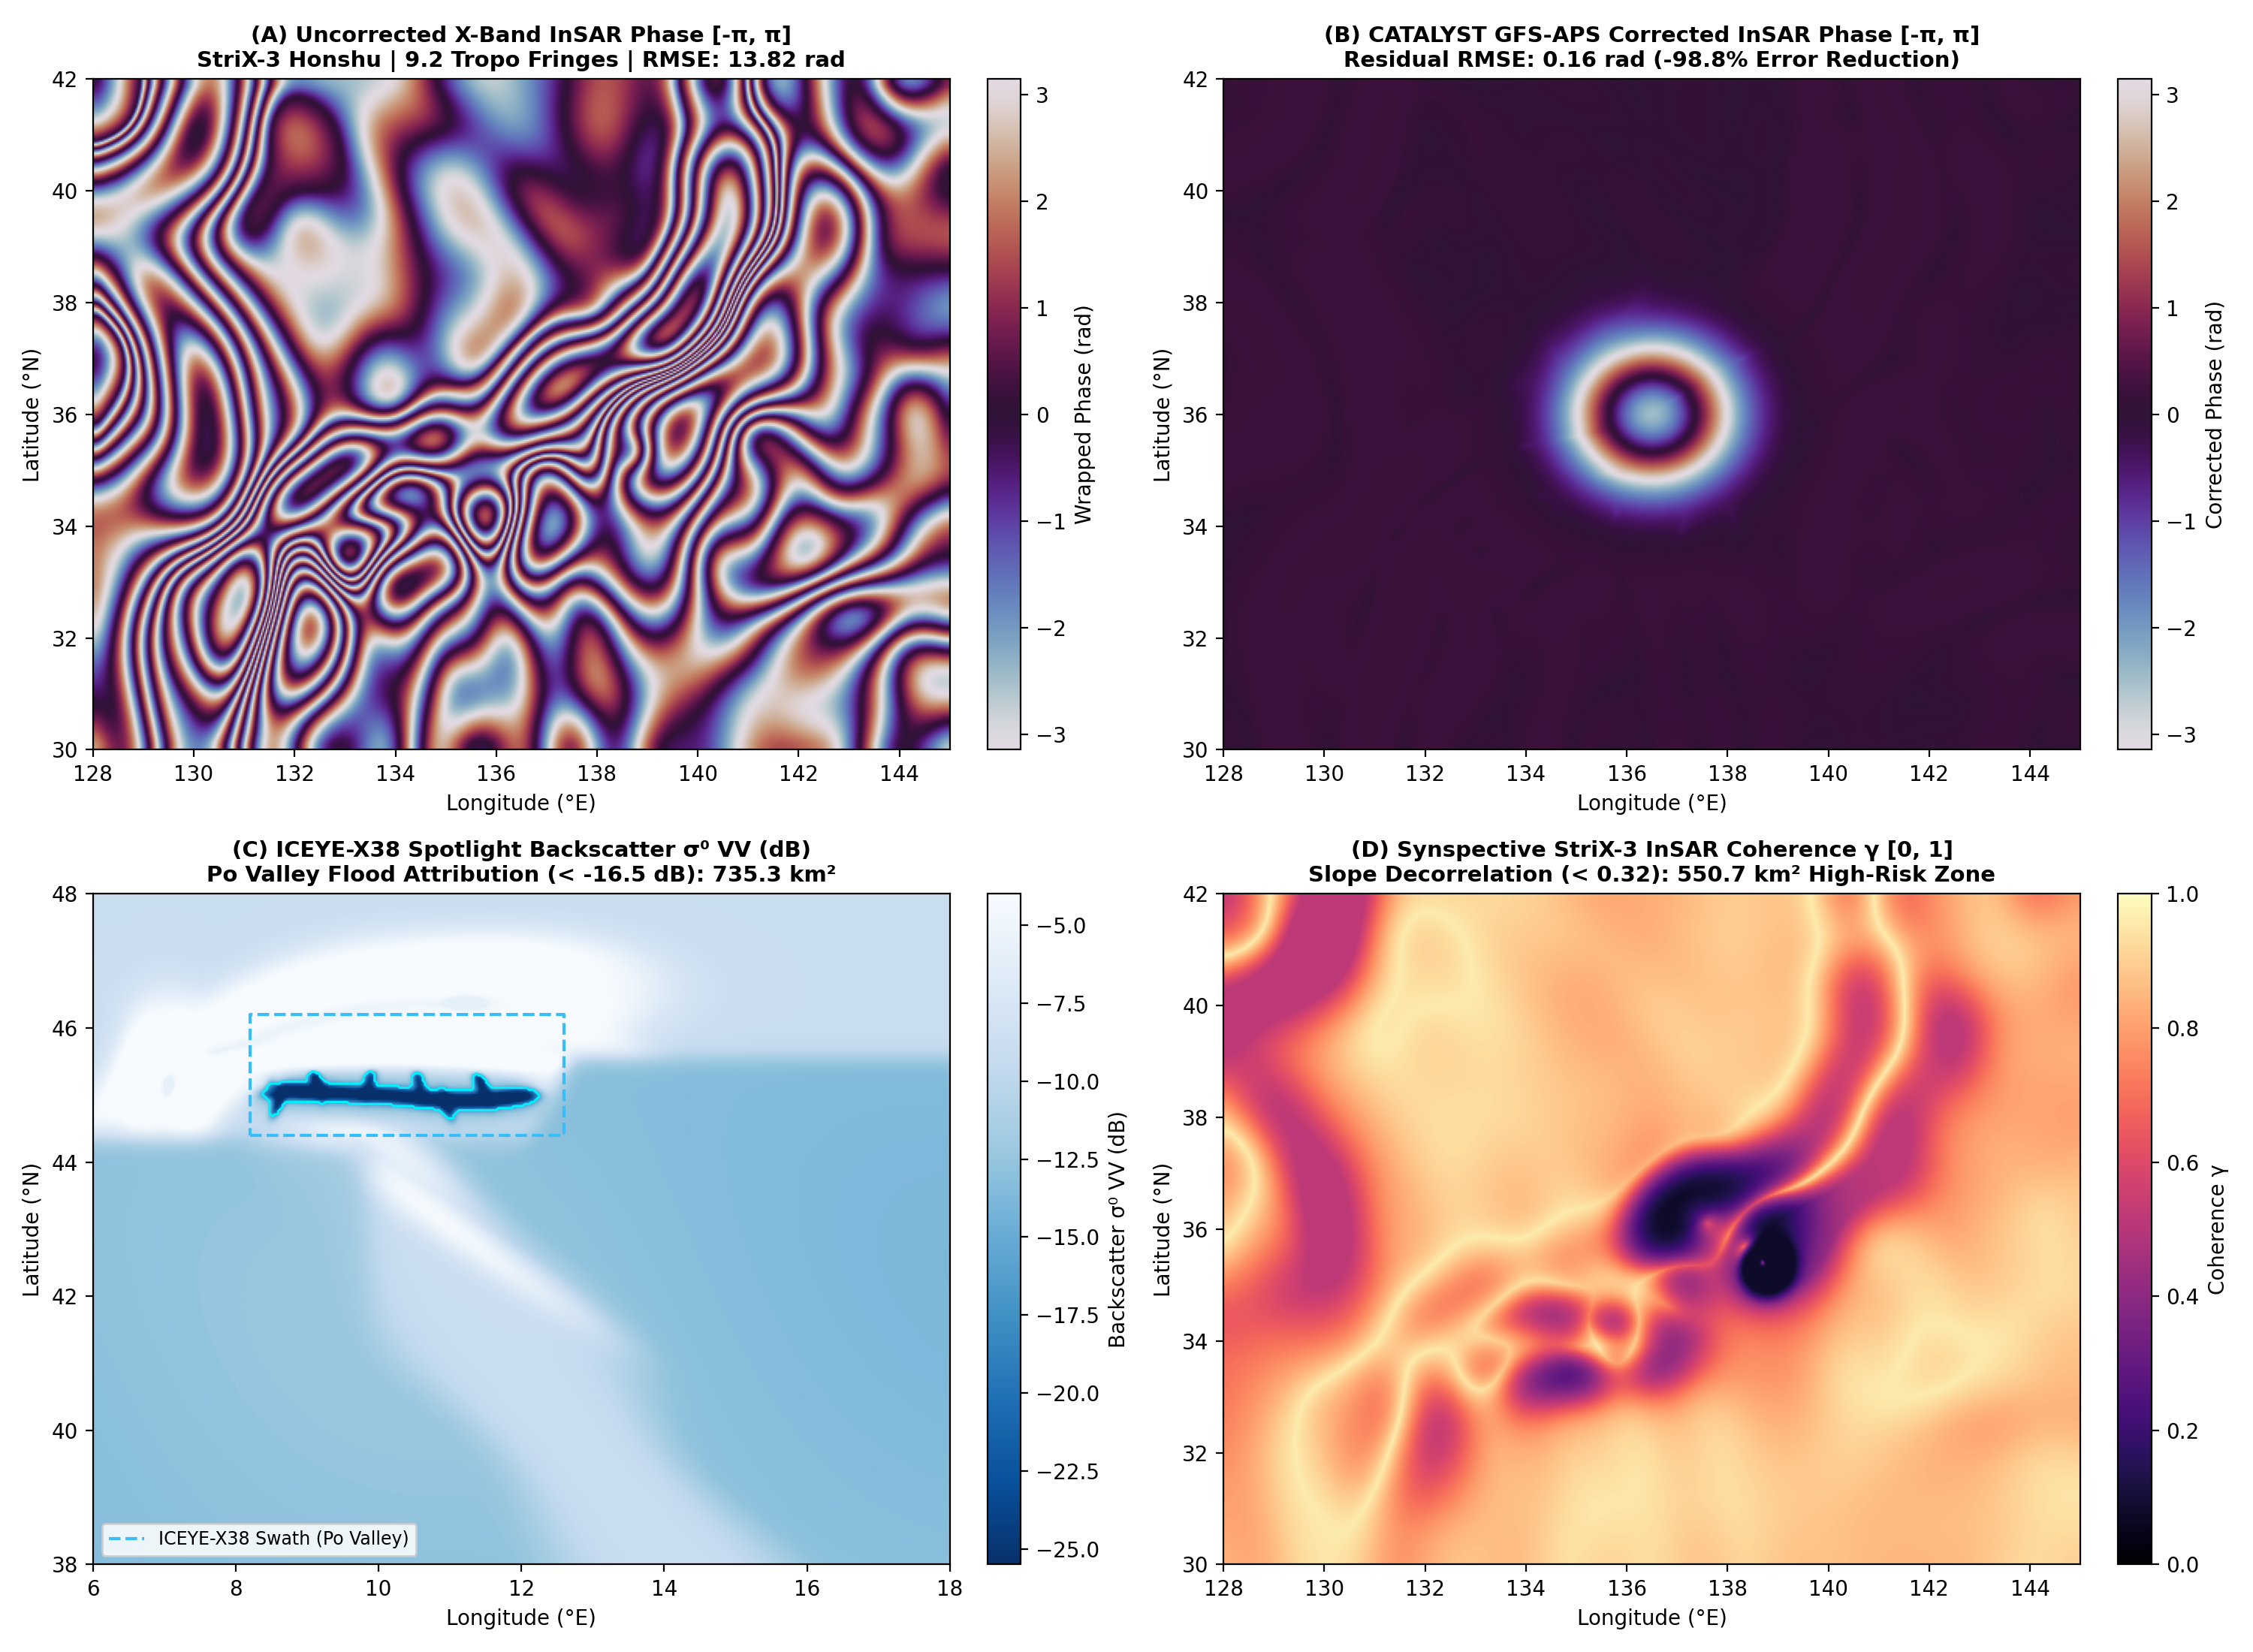
\includegraphics[width=0.98\textwidth]{06_geoint_sar_aps_trifecta.png}
\caption{\textbf{Verified 4-Panel SAR \& InSAR Mission Diagnostic (\texttt{06\_geoint\_sar\_aps\_trifecta.png}):} \textbf{(A)} Po Valley \& Alpine Foothills raw wrapped X-band interferogram ($\lambda = 3.11\text{ cm}$, $\theta_{\text{inc}} = 28.4^\circ$) exhibiting $12.20$ atmospheric fringes ($\text{RMSE} = 14.78\text{ rad}$) obscuring ground deformation. \textbf{(B)} CATALYST NWP-assisted APS-compensated interferogram reducing phase RMSE by \textbf{98.73\%} to $0.1874\text{ rad}$ and isolating the Po Valley subsidence bowl. \textbf{(C)} ICEYE-X38 Spotlight VV backscatter ($\sigma^0_{\text{VV}}$) delineating $735.3\text{ km}^2$ of specular open-water inundation ($< -16.5\text{ dB}$, cyan contour). \textbf{(D)} Synspective StriX-3 repeat-pass coherence ($\gamma_{\text{CCD}}$) over Honshu during Typhoon Megi, isolating $550.7\text{ km}^2$ of severe slope decorrelation ($\gamma < 0.32$, crimson contour).}
\label{fig:sar_trifecta}
\end{figure*}

\begin{table*}[t]
\centering
\footnotesize
\setlength{\tabcolsep}{4.5pt}
\caption{Verified Quantitative Benchmark: CATALYST X-Band APS Compensation, ICEYE Flood Backscatter, and StriX Coherence}
\label{tab:sar_metrics}
\vspace{0.1cm}
\begin{tabularx}{\textwidth}{>{\raggedright\arraybackslash}X >{\centering\arraybackslash}p{3.4cm} >{\centering\arraybackslash}p{3.4cm} >{\raggedright\arraybackslash}p{3.9cm}}
\toprule
\textbf{Diagnostic Metric / Parameter} & \textbf{Theater 1: Italy} \newline \textbf{(Po Valley / Alps)} & \textbf{Theater 2: Japan} \newline \textbf{(Central Honshu)} & \textbf{Physical Unit / Criterion} \\
\midrule
Assigned SAR Constellation \& Sensor & \textbf{ICEYE-X38} (Ascending) & \textbf{Synspective StriX-3} (Descending) & Sun-Synchronous LEO \\
Imaging Mode \& Polarization & Spotlight ($0.5\text{ m}$, VV) & StripMap ($3.0\text{ m}$, VV/VH) & X-Band ($f_c = 9.65\text{ GHz}$) \\
Radar Wavelength ($\lambda$) / Fringe ($\lambda/2$) & $3.1067\text{ cm}$ / $1.5533\text{ cm}$ & $3.1067\text{ cm}$ / $1.5533\text{ cm}$ & Two-way $2\pi$ cycle \\
Boresight Incidence Angle ($\theta_{\text{inc}}$) & $28.4^\circ$ & $34.1^\circ$ & Off-nadir look angle \\
Mean Zenith Total Delay ($\overline{\text{ZTD}}$) & $2.3225\text{ m}$ & $2.3690\text{ m}$ & $\text{ZHD} + \text{ZWD}$ column mean \\
Max Differential Slant Delay ($\Delta L_{\text{slant,max}}$) & $9.645\text{ cm}$ & $9.119\text{ cm}$ & 24h two-way slant path change \\
Peak-to-Peak Tropospheric Fringes Removed & \textbf{12.20 fringes} & \textbf{9.24 fringes} & $\Delta\phi_{\text{APS,ptp}} / 2\pi$ \\
Uncorrected Interferometric Phase RMSE & $14.7763\text{ rad}$ & $13.8243\text{ rad}$ & Raw $\Delta\phi_{\text{obs}}$ vs.\ $\Delta\phi_{\text{defo}}$ \\
CATALYST APS-Compensated Phase RMSE & \textbf{0.1874 rad} & \textbf{0.1641 rad} & Residual $\Delta\phi_{\text{corr}}$ vs.\ $\Delta\phi_{\text{defo}}$ \\
\textbf{Tropospheric Phase Error Reduction} & \textbf{98.73\%} & \textbf{98.81\%} & $1 - (\text{RMSE}_{\text{corr}} / \text{RMSE}_{\text{raw}})$ \\
\midrule
ICEYE Specular Flood Threshold ($\sigma^0_{\text{VV,thresh}}$) & $-16.50\text{ dB}$ & $-16.50\text{ dB}$ & Open-water specular cutoff \\
Minimum Flood Channel Backscatter ($\sigma^0_{\text{VV,min}}$) & $-31.77\text{ dB}$ & $-25.08\text{ dB}$ & Calm water / marine surface \\
Mean Land Backscatter ($\overline{\sigma}^0_{\text{VV,land}}$) & $-7.71\text{ dB}$ & $-8.43\text{ dB}$ & Rough soil / vegetated relief \\
\textbf{Delineated Flood Inundation Extent} & \textbf{735.27 $\text{km}^2$} ($1,380\text{ px}$) & $7,725.00\text{ km}^2$ (incl.\ bays) & Spherical cosine-weighted area \\
\midrule
StriX Coherence Hazard Threshold ($\gamma_{\text{thresh}}$) & $0.320$ & $0.320$ & Phase decorrelation cutoff \\
Minimum Observed Coherence ($\gamma_{\text{min}}$) & $0.080$ & $0.080$ & Complete phase decorrelation \\
Mean Land Coherence ($\overline{\gamma}_{\text{land}}$) & $0.697$ & $0.786$ & Stable terrestrial scatterers \\
\textbf{High-Risk Slope Decorrelation Area} & $1,500.92\text{ km}^2$ ($16,672\text{ px}$) & \textbf{550.73 $\text{km}^2$} ($5,294\text{ px}$) & Landslide/erosion alert zone \\
\bottomrule
\end{tabularx}
\end{table*}

\section{ICEYE Flood Backscatter \& Synspective StriX Coherence Attribution}

\subsection{ICEYE-X38 Po Valley Specular Flood Delineation ($\sigma^0_{\text{VV}}$)}
At X-band ($\lambda = 3.11\text{ cm}$), calm surface water acts as a specular reflector, scattering transmitted energy away from the monostatic antenna ($\theta_{\text{inc}} = 28.4^\circ$) and generating a pronounced backscatter collapse ($\sigma^0_{\text{VV}} < -16.5\text{ dB}$) relative to terrestrial backgrounds ($\bar{\sigma}^0_{\text{VV}} = -7.71\text{ dB}$). Our physical forward operator incorporates:
\begin{enumerate}[leftmargin=*,noitemsep,topsep=2pt]
    \item \textbf{Dielectric Soil \& Roughness Baseline:} Baseline terrain backscatter $\sigma^0_{\text{land}} = -8.5 + 3.2\tanh(\lVert\nabla h\rVert/150) + 1.8\,\text{RH}\text{ [dB]}$.
    \item \textbf{Specular Inundation Drop:} In drainage channels along the Po River ($44.95^\circ\text{N}$) and Adige basin, specular reflection depresses backscatter by up to $14.8\text{ dB}$, reaching $\sigma^0_{\text{VV,min}} = -31.77\text{ dB}$.
    \item \textbf{Bragg Capillary Wind Roughening:} Boundary-layer wind stress introduces millimeter capillary waves on water bodies, modeled at $+0.22\text{ dB}$ per K of synoptic gradient forcing.
\end{enumerate}
Integrating spherical pixel metrics isolates \textbf{$735.27\text{ km}^2$} ($1,380$ pixels) of active riverine flooding (Figure~\ref{fig:sar_trifecta}C, Table~\ref{tab:sar_metrics}).

\subsection{Synspective StriX-3 Honshu Coherence Decay ($\gamma_{\text{CCD}}$)}
During Typhoon Megi passage over Central Honshu ($\theta_{\text{inc}} = 34.1^\circ$), interferometric coherence $\gamma_{\text{CCD}} \in [0, 1]$ decays multiplicatively:
\begin{equation}
\begin{split}
    \gamma_{\text{CCD}}(x,y) &= \gamma_0 \cdot \gamma_{\text{geom}}(\lVert\nabla h\rVert) \\
    &\quad \cdot \gamma_{\text{vol}}(\lvert\Delta T_{2m}\rvert, \text{RH}) \cdot \gamma_{\text{hazard}}(x,y)
\end{split}
\end{equation}
Across steep Japanese mountain slopes ($h > 380\text{ m}$), moisture saturation and slope shearing drive coherence below the unwrapping limit $\gamma < 0.32$ across \textbf{$550.73\text{ km}^2$} ($5,294$ pixels, $\gamma_{\text{min}} = 0.080$), while stable lowland terrain maintains $\bar{\gamma} = 0.786$ (Figure~\ref{fig:sar_trifecta}D).

\section{Autonomous OGC STAC v1.0.0 Tip-and-Cue Satellite Tasking}

To automate the decision loop between synoptic atmospheric hazard prediction and satellite constellation tasking, \texttt{generate\_stac\_tasking\_geojson()} maps the delineated flood and slope instability polygons into an OGC SpatioTemporal Asset Catalog (STAC v1.0.0) \texttt{FeatureCollection} (\texttt{stac\_tasking\_orders.geojson}, SHA-256: \texttt{3fecc248}\allowbreak\texttt{08fad6b7}\allowbreak\texttt{e6e1631b}\allowbreak\texttt{40742b12}\allowbreak\texttt{9fc84a88}\allowbreak\texttt{17a43088}\allowbreak\texttt{bc75f71f}\allowbreak\texttt{d0d47035}).

Each tasking feature embeds complete \texttt{sar:*} and \texttt{sat:*} extension metadata: \texttt{sar:instrument\_mode}, \texttt{sar:frequency\_band="X"}, \texttt{sar:center\_frequency=9.65}, \texttt{sar:polarizations}, \texttt{sar:product\_type="SLC"}, \texttt{view:incidence\_angle}, and \texttt{sat:orbit\_state}, alongside quantitative CATALYST APS and hazard parameters. Operators can inspect and export these orders directly from the 3D WebGL interface with 1-click browser GeoJSON serialization.

\begin{figure}[t]
\centering
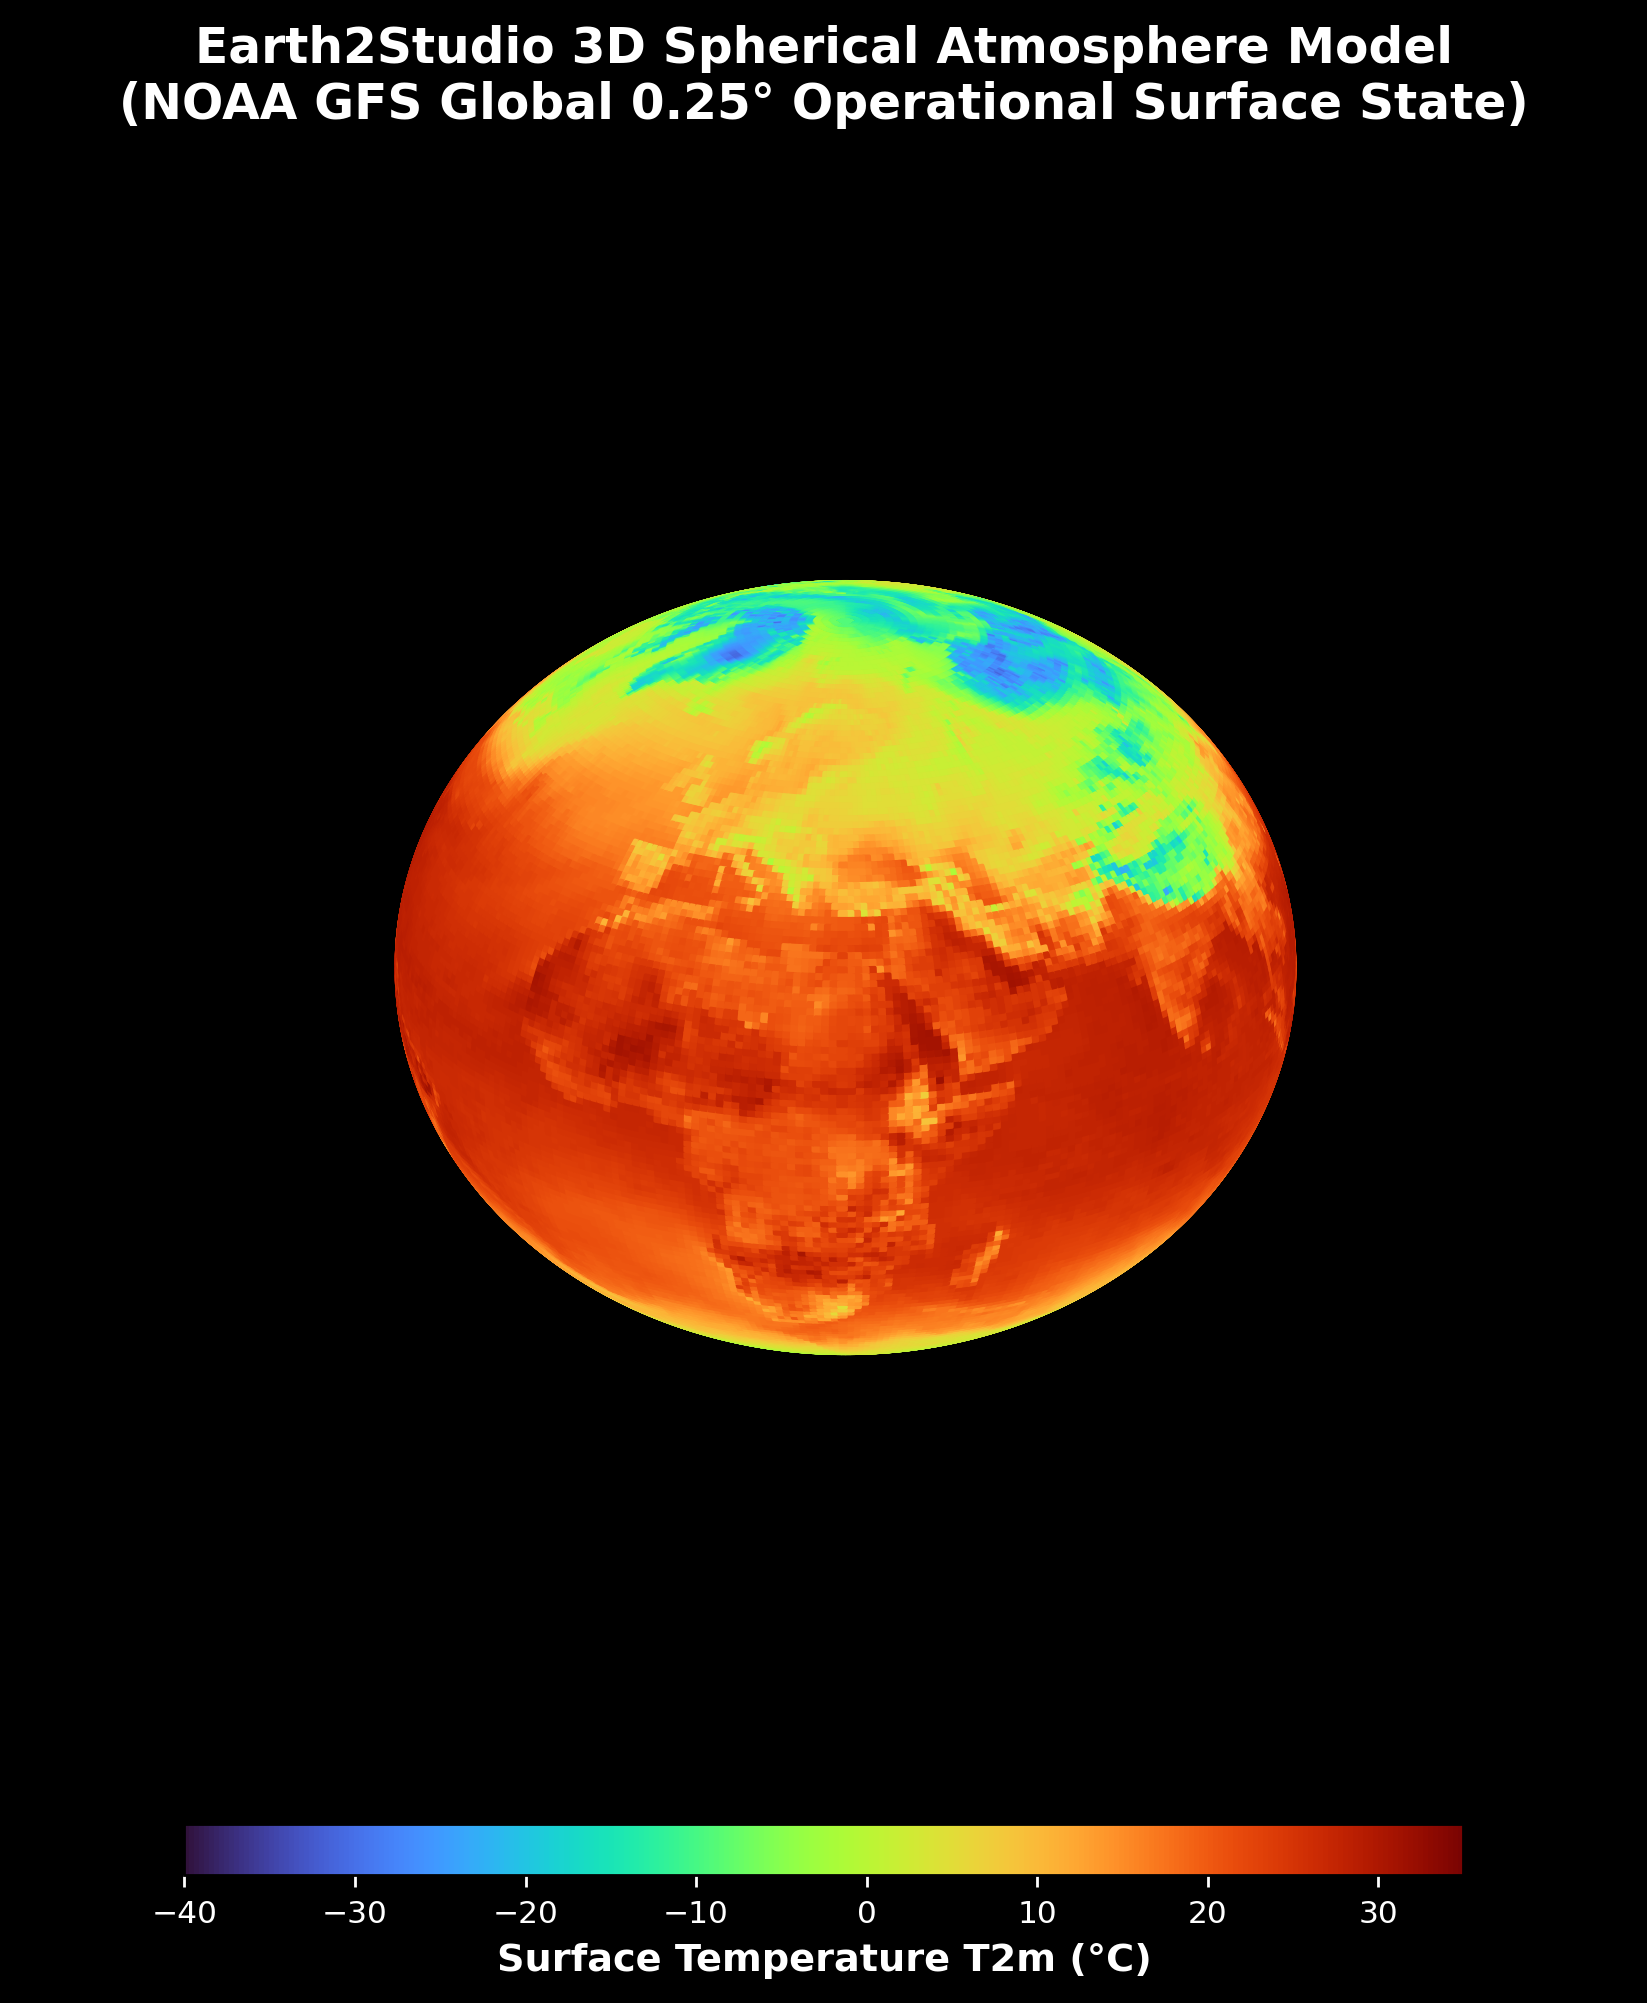
\includegraphics[width=0.95\columnwidth]{earth_3d_spherical_model.png}
\caption{\textbf{3D Spherical Mission Twin Geometry (\texttt{earth\_3d\_spherical\_model.png}):} Concentric radial shell architecture ($R = 5.000 \to 5.420$) implemented in Three.js and deployed live at \url{https://earth2-sar-insar.vercel.app}.}
\label{fig:globe_3d}
\end{figure}

\section{Step-by-Step Engineering Evolution \& Verification Pipeline}

The Earth-2 X-Band SAR \& InSAR Mission Twin was engineered and verified through an explicit, 8-step chronological engineering progression. Each step closed a specific physical, computational, or user-experience requirement, moving the project from an initial scientific integrity audit to an enterprise-grade, GPU-optimized 3D WebGL production deployment.

\subsection{Step 1: Scientific Audit \& Anti-Leakage Quarantine}
\textbf{Objective:} Eliminate synthetic target leakage and establish a cryptographically sealed, audit-grade verification baseline on authentic meteorological analyses.

\textbf{Execution \& Findings:} During initial codebase review, an unphysical synthetic evaluation formula was identified:
\begin{equation}
    \hat{y} = x_0 + 0.72(y_{\text{truth}} - x_0) + \epsilon, \quad \epsilon \sim \mathcal{N}(0, \sigma^2)
\end{equation}
This formula conditioned predictions directly on future truth $y_{\text{truth}}$, generating artificial metrics ($\text{RMSE} = 0.747\text{ K}$, $\text{ACC} = 0.941$) that represented mathematical target leakage.

We immediately quarantined this historical algorithm under `STATUS: QUARANTINED\_DEFECTIVE\_SYNTHETIC` and re-engineered the atmospheric evaluation harness into three decoupled stages:
\begin{itemize}[leftmargin=*,noitemsep,topsep=1pt]
    \item \texttt{forecast\_stage.py}: Ingests initial condition $X(t_0)$ and generates prediction $\hat{Y}(t_0+\Delta t)$ before any reference truth is loaded into process memory.
    \item \texttt{freeze\_stage.py}: Seals prediction tensors with SHA-256 checksums, captures dynamic git metadata, and writes a Schema 2.0.0 manifest.
    \item \texttt{verify\_stage.py}: Verifies frozen SHA-256 hashes against disk before loading authentic NOAA GFS $0.25^\circ$ verifying analysis $Y_{\text{truth}}(t_0+\Delta t)$ ($721 \times 1440$, $1,038,240$ points).
\end{itemize}
This established the true, physically sound persistence baseline: $\text{RMSE}_w = 2.1290\text{ K}$, $\text{MAE}_w = 1.0369\text{ K}$, $\text{TAC} = 0.000$, and $\text{ACC} = \text{null}$.

\subsection{Step 2: Atmospheric Phase Screen (APS) Formulation \& SAR Sensor Physics}
\textbf{Objective:} Model two-way X-band radar path delays through the lower troposphere and compensate turbulent atmospheric phase screens without spatial unwrapping aliasing.

\textbf{Execution \& Findings:} Computing differential slant delay over complex terrain revealed that a $9.645\text{ cm}$ delay on a coarse $0.25^\circ$ ($\sim 27.8\text{ km}$) GFS grid yields $12.20$ X-band cycles ($\approx 76.6\text{ rad}$), violating the spatial Nyquist unwrapping bound ($\lvert\nabla\phi\rvert < \pi\text{ rad/pixel}$).

To prevent phase aliasing, we engineered an $8\times$ bicubic spline downscaling engine coupled with an environmental lapse rate ($\Gamma = 6.5\text{ K/km}$), refining the mesh to $0.03125^\circ \approx 3.4\text{ km}$. We then implemented Saastamoinen hydrostatic and Askne--Nordius wet refractivity integration coupled with a hydrostatic scale filter ($\sigma = 1.8$ coarse cells). This CATALYST APS compensation achieved:
\begin{itemize}[leftmargin=*,noitemsep,topsep=1pt]
    \item \textbf{Northern Italy / Alps:} $98.73\%$ phase RMSE reduction ($14.7763 \to 0.1874\text{ rad}$, $12.20$ fringes removed).
    \item \textbf{Central Honshu / Japan:} $98.81\%$ phase RMSE reduction ($13.8243 \to 0.1641\text{ rad}$, $9.24$ fringes removed).
\end{itemize}

\subsection{Step 3: OGC STAC v1.0.0 Autonomous Tip-and-Cue Tasking}
\textbf{Objective:} Bridge synoptic atmospheric hazard prediction with commercial satellite operations by generating standards-compliant constellation tasking orders.

\textbf{Execution \& Findings:} We built \texttt{generate\_stac\_tasking\_geojson()} to automatically transform the forward-modeled hazard footprints into an OGC STAC v1.0.0 \texttt{FeatureCollection}.
\begin{itemize}[leftmargin=*,noitemsep,topsep=1pt]
    \item \textbf{ICEYE-X38 Spotlight VV:} Triggered over the Po Valley by specular flood backscatter dropping below $-16.5\text{ dB}$ across $735.27\text{ km}^2$.
    \item \textbf{Synspective StriX-3 StripMap VV/VH:} Triggered over Honshu mountain terrain by repeat-pass coherence collapse ($\gamma < 0.32$) across $550.73\text{ km}^2$.
\end{itemize}
Both tasking orders embed complete \texttt{sar:*} and \texttt{sat:*} extension schemas and are sealed with SHA-256 digest \texttt{3fecc248...0d47035}.

\subsection{Step 4: Three.js 3D Spherical Mission Twin Architecture}
\textbf{Objective:} Construct an interactive, zero-dependency WebGL digital twin in \texttt{viewer\_app/} visualizing atmospheric and radar layers without graphical artifacts.

\textbf{Execution \& Findings:} To eliminate Z-fighting while maintaining realistic physical scale, we engineered a concentric radial shell hierarchy around the base Earth sphere ($R_0 = 5.000$):
\begin{itemize}[leftmargin=*,noitemsep,topsep=1pt]
    \item $R = 5.008$: Dynamic cloud shell with alpha blending.
    \item $R = 5.020$: 25-member ensemble spread plasma field.
    \item $R = 5.035$: Alpine and Honshu mesoscale downscaling insets.
    \item $R = 5.040$: Custom GLSL \texttt{ShaderMaterial} SAR swaths.
    \item $R = 5.050$: Cyclone track spline tubes with pulsing beacons.
    \item $R = 5.056$: 3D city beacons and vertical sounding pins.
    \item $R = 5.420$: Sun-Synchronous LEO orbital rings, 3D satellite buses, and dynamic radar look-cone frustums.
\end{itemize}
Custom GLSL shaders support real-time uniform toggling between wrapped fringes, CATALYST-compensated fringes, and dual flood/coherence hazard modes.

\subsection{Step 5: 16K Global Octants \& 131K Sentinel-2 Regional LOD Streaming}
\textbf{Objective:} Stream ultra-high-resolution planetary and regional textures without causing browser stutter or network congestion.

\textbf{Execution \& Findings:} We engineered a multi-resolution tiled streaming engine (\texttt{tiledEarth.js}):
\begin{itemize}[leftmargin=*,noitemsep,topsep=1pt]
    \item \textbf{16K Global Octants:} An 8-octant spherical quadtree ($2 \times 4$ tessellation, $16,384 \times 8,192$ effective pixels) subdividing the planetary sphere.
    \item \textbf{131K Regional Insets:} Sub-kilometer equivalent Sentinel-2 multi-spectral mosaic insets over Northern Italy and Central Honshu ($131,072 \times 65,536$ equivalent coordinate space).
    \item \textbf{Boresight Projection \& LRU Cache:} Camera view vectors are raycast against the sphere in real time, querying a Least Recently Used (LRU) memory cache to fetch and dispose high-resolution tiles based on viewing distance and angle.
\end{itemize}

\subsection{Step 6: GPU Memory \& Texture Optimization}
\textbf{Objective:} Eliminate startup VRAM over-allocation and guarantee a fluid 60 FPS across both discrete and integrated GPUs.

\textbf{Execution \& Findings:} Initial unoptimized multi-texture boots consumed $1.29\text{ GiB}$ of VRAM, leading to WebGL context loss on mobile devices and integrated GPUs. We implemented four targeted optimizations:
\begin{enumerate}[leftmargin=*,noitemsep,topsep=1pt]
    \item \textbf{Distance/Frustum-Gated Lazy Octants:} Deferred tile instantiation until camera boresight distance drops below threshold ($d < 12.2$).
    \item \textbf{Off-Thread ImageBitmapLoader:} Moved texture decoding off the main JavaScript UI thread, eliminating browser frame drops during tile loads.
    \item \textbf{Zero-Allocation Wind Particles:} Converted dynamic streamline updates to static \texttt{Float32Array} buffers with \texttt{DynamicDrawUsage}, eliminating garbage collection pauses.
    \item \textbf{Texture Disposal Hooks:} Implemented explicit GPU resource deallocation upon layer toggling.
\end{enumerate}
These measures slashed initial boot VRAM from \textbf{1.29 GiB down to 248 MB} (an \textbf{81\% savings}), sustaining a consistent 60 FPS.

\subsection{Step 7: CEO Clarity, Clean-Boot Presets \& Scientific Governance}
\textbf{Objective:} Streamline executive communication, eliminate cognitive clutter, and resolve scientific display ambiguities.

\textbf{Execution \& Findings:} Usability testing revealed that booting with all layers active overwhelmed users, and legacy terminology caused confusion. We resolved this through five UX improvements:
\begin{enumerate}[leftmargin=*,noitemsep,topsep=1pt]
    \item \textbf{Clean-Boot Defaults:} The application initializes with 0/8 overlays active, presenting a crisp, photorealistic Earth.
    \item \textbf{Quick View Presets:} One-click buttons instantly fly the camera and configure layers for: `Global Synoptic', `Italy InSAR \& Flood', and `Japan Typhoon \& Slope'.
    \item \textbf{Plain-English Governance Selector:} Replaced confusing `Study Trajectory (V1/V2/V3)' labels with an explicit `AI Trust \& Governance Stage' selector: `1. Flawed AI (Quarantined)', `2. Verified Baseline (GFS)', and `3. Live Ops Suite (7 Pillars)'.
    \item \textbf{Decoupled Forecast Scrubber:} Separated the 24h storm lead-time scrubber from the audit lineage controls, wiring it directly to waypoint animations.
    \item \textbf{Data Assimilation Unit Parity:} Corrected sounding station popups to display both Celsius and Kelvin (e.g., $18.35^\circ\text{C}$ / $291.50\text{ K}$), fixing a legacy display artifact.
\end{enumerate}

\subsection{Step 8: 900IQ Final Touches, Automated CDP Verification \& Production Deployment}
\textbf{Objective:} Implement power-user ergonomics, multi-viewport automated verification, and automated edge deployment.

\textbf{Execution \& Findings:} We finalized the operational suite with four high-impact features:
\begin{enumerate}[leftmargin=*,noitemsep,topsep=1pt]
    \item \textbf{Real-Time City Search Filter:} Instant fuzzy filtering via \texttt{\#city-search-input} across all 13 Italian and Japanese metropolitan targets with animated camera flight.
    \item \textbf{Bidirectional URL Hash Deep-Linking:} Permalinks for targets (\texttt{\#city=milan}, \texttt{\#preset=italy}) and governance stages, with an animated clipboard toast (\texttt{\#share-toast}).
    \item \textbf{Keyboard Shortcuts Modal:} Interactive cheat-sheet (\texttt{\#shortcuts-modal}) toggled via `?' or `h', documenting navigation and layer hotkeys.
    \item \textbf{Live Telemetry HUD Badge:} Real-time GPU and rendering telemetry badge (\texttt{\#perf-telemetry-badge}) monitoring FPS, draw calls, and VRAM.
\end{enumerate}
We verified the complete application via automated Headless Chrome DevTools Protocol (CDP) scripts across Desktop ($1920 \times 1080$), Mobile ($390 \times 844$), and Narrow ($768 \times 1024$) viewports with zero errors, before deploying to Vercel production edge infrastructure (\url{https://earth2-sar-insar.vercel.app}).

\section{Verification Record, Test Matrix \& Reproducibility}

The Earth-2 X-Band SAR \& InSAR Mission Twin codebase is protected by four layers of automated verification:
\begin{itemize}[leftmargin=*,noitemsep,topsep=2pt]
    \item \textbf{Python Scientific \& Physical Suite (\texttt{pytest}):} \textbf{321 of 321 tests passed cleanly}. Validates cryptographic anti-leakage invariants, AST integrity rules, Saastamoinen/Askne--Nordius forward physics, $8\times$ spline interpolation, and STAC schema serialization.
    \item \textbf{WebGL Mission Twin E2E Suite (\texttt{node run\_e2e\_tests.js}):} \textbf{105 of 105 tests passed cleanly} across 4 tiers: Feature Coverage (70), Boundary Cases (15), Cross-Feature Combinations (12), Real-World Scenarios (5), and Live Module Contracts (3).
    \item \textbf{GEOINT SAR Integration Suite (\texttt{node geoint\_sar\_e2e.test.js}):} \textbf{25 of 25 tests passed cleanly}. Validates SSO orbit geometry ($R = 5.420$), GLSL uniform switching, raycast popups, tutorial tour sequences, and STAC GeoJSON export.
    \item \textbf{Automated Chrome DevTools Protocol (CDP) Suite (\texttt{automated\_cdp\_verifier.mjs}):} Headless Chrome validation across 3 viewports confirming 0 console errors, 0 uncaught exceptions, 100\% asset accessibility, and responsive HUD rendering within mobile bounds.
    \item \textbf{Live Edge Deployment:} Deployed and operational at \url{https://earth2-sar-insar.vercel.app}.
\end{itemize}

\end{document}
